% Options for packages loaded elsewhere
\PassOptionsToPackage{unicode}{hyperref}
\PassOptionsToPackage{hyphens}{url}
%
\documentclass[
  14pt,
]{article}
\usepackage{amsmath,amssymb}
\usepackage{iftex}
\ifPDFTeX
  \usepackage[T1]{fontenc}
  \usepackage[utf8]{inputenc}
  \usepackage{textcomp} % provide euro and other symbols
\else % if luatex or xetex
  \usepackage{unicode-math} % this also loads fontspec
  \defaultfontfeatures{Scale=MatchLowercase}
  \defaultfontfeatures[\rmfamily]{Ligatures=TeX,Scale=1}
\fi
\usepackage{lmodern}
\ifPDFTeX\else
  % xetex/luatex font selection
\fi
% Use upquote if available, for straight quotes in verbatim environments
\IfFileExists{upquote.sty}{\usepackage{upquote}}{}
\IfFileExists{microtype.sty}{% use microtype if available
  \usepackage[]{microtype}
  \UseMicrotypeSet[protrusion]{basicmath} % disable protrusion for tt fonts
}{}
\makeatletter
\@ifundefined{KOMAClassName}{% if non-KOMA class
  \IfFileExists{parskip.sty}{%
    \usepackage{parskip}
  }{% else
    \setlength{\parindent}{0pt}
    \setlength{\parskip}{6pt plus 2pt minus 1pt}}
}{% if KOMA class
  \KOMAoptions{parskip=half}}
\makeatother
\usepackage{xcolor}
\usepackage[margin=1in]{geometry}
\usepackage{longtable,booktabs,array}
\usepackage{calc} % for calculating minipage widths
% Correct order of tables after \paragraph or \subparagraph
\usepackage{etoolbox}
\makeatletter
\patchcmd\longtable{\par}{\if@noskipsec\mbox{}\fi\par}{}{}
\makeatother
% Allow footnotes in longtable head/foot
\IfFileExists{footnotehyper.sty}{\usepackage{footnotehyper}}{\usepackage{footnote}}
\makesavenoteenv{longtable}
\usepackage{graphicx}
\makeatletter
\newsavebox\pandoc@box
\newcommand*\pandocbounded[1]{% scales image to fit in text height/width
  \sbox\pandoc@box{#1}%
  \Gscale@div\@tempa{\textheight}{\dimexpr\ht\pandoc@box+\dp\pandoc@box\relax}%
  \Gscale@div\@tempb{\linewidth}{\wd\pandoc@box}%
  \ifdim\@tempb\p@<\@tempa\p@\let\@tempa\@tempb\fi% select the smaller of both
  \ifdim\@tempa\p@<\p@\scalebox{\@tempa}{\usebox\pandoc@box}%
  \else\usebox{\pandoc@box}%
  \fi%
}
% Set default figure placement to htbp
\def\fps@figure{htbp}
\makeatother
\setlength{\emergencystretch}{3em} % prevent overfull lines
\providecommand{\tightlist}{%
  \setlength{\itemsep}{0pt}\setlength{\parskip}{0pt}}
\setcounter{secnumdepth}{-\maxdimen} % remove section numbering
\usepackage{bookmark}
\IfFileExists{xurl.sty}{\usepackage{xurl}}{} % add URL line breaks if available
\urlstyle{same}
\hypersetup{
  pdftitle={DC's tipped minimum wage: Exploring the economic debate},
  pdfauthor={Leah Roffman},
  hidelinks,
  pdfcreator={LaTeX via pandoc}}

\title{DC's tipped minimum wage: Exploring the economic debate}
\author{Leah Roffman}
\date{2025-06-19}

\begin{document}
\maketitle

\section{Introduction}\label{introduction}

It can sometimes be hard to look away from a good argument on Twitter. I
recently came across this one, where a nonprofit director tears into
graphs from a DC Budget Council report:\footnote{\url{https://x.com/Mike_Saltsman/status/1929562788214510054}}

\begin{center}\includegraphics[width=0.5\linewidth,height=0.5\textheight]{./Images/TwitterScreenshot} \end{center}

\emph{Source =
\url{https://x.com/Mike_Saltsman/status/1929562788214510054}}

Looking into the details, you'll find that the nonprofit director is the
Executive Director of the Employment Policies Institute, and what
they're contesting is the impact of DC's tipped minimum wage policy --
Initiative 82.

Initiative 82 (I82) was first passed in 2022, after a ballot initiative
for raising the tipped minimum wage in the District received 73.9\% of
the popular vote. At the time, the DC minimum wage for service workers
was only \$5.35/hr, well below the standard minimum wage of \$16.10/hr
(now up to \$17.50/hr).\footnote{\url{https://fred.stlouisfed.org/series/STTMINWGDC}}
Although service workers do make tips on top of their base wages, tips
are dependent on customer spending levels and generosity, leading to
cases of income instability.

Under I82, the tipped minimum wage has already been increased to \$10,
with further increases planned in coming years. However, despite initial
popular support, the DC Council voted to pause I82 implementation in
June of this year.\footnote{Jackie Bensen, ``DC Council votes to pause
  voter-approved tipped wage increase'', \emph{NBC},
  \url{https://www.nbcwashington.com/news/local/dc-council-votes-to-pause-tipped-wage-increase/3927718/}}
As evidenced by the Tweet exchange, many of I82's impacts have been
heavily contested, with enough concern that Mayor Muriel Bowser has even
proposed repealing the policy completely.

Groups like the \href{https://epionline.org/}{Employment Policies
Institute (EPI)} and the \href{https://www.ramw.org/}{Restaurant
Association of Metropolitan Washington (RAMW)} have argued that I82 is
adding untenable stress to the local economy. According to their data
and surveys, both the restaurant industry and service workers are
hurting under the policy. Not to mention, there have been high-profile
restaurant closures, with many restaurants expressing concerns about
additional closures in 2025.\footnote{Jessica Sidman, ``How Much Trouble
  Are DC Restaurants Really In?'', \emph{The Washingtonian},
  \url{https://www.washingtonian.com/2025/04/03/how-much-trouble-are-dc-restaurants-really-in/}}

At the same time, the service workers' union
\href{https://x.com/UHLocal25/status/1929508002828042472}{Unite Local
25} and the advocacy group
\href{https://static1.squarespace.com/static/6374f6bf33b7675afa750d48/t/65551d0897043249c7c1293b/1700076810648/OFW_OneYearAfter_DC82+\%281\%29.pdf}{One
Fair Wage} have argued that there is a lack of economic evidence showing
that the industry is suffering due to I82. The DC Budget Council, a
research body for DC's councilmembers, appears to support this premise.
Their recent report showed healthy trends in employment levels, income,
and restaurant growth since 2022.

It makes sense why restaurant owners and service workers may have
contradictory views on how the policy has played out. But why does their
data differ -- and what evidence should drive the DC Council's decision
on whether or not to keep the policy?

Without diving into every piece of this complex issue, I was curious to
take a closer look at some of the charts I saw on Twitter.

\section{Data exploration and
analysis}\label{data-exploration-and-analysis}

\subsection{What are the impacts being
debated?}\label{what-are-the-impacts-being-debated}

I82 was officially implemented in May 2023, so any effects will have
emerged in a somewhat short timeframe.

The initial wage increases under the policy have followed a staggered
format. There have been increases from \$5.35 to \$6.00, \$6.00 to
\$8.00, and most recently, \$8.00 to \$10.00 in July 2024. Under the
timeline, the tipped minimum wage would reach standard DC minimum wage
by 2027. However, with the DC Council voting to pause implementation,
the next planned increase from \$10.00 to \$12.00 has been temporarily
halted.

We still have a small timeframe of data from which to try and analyze
the policy's impact. Raising the tipped minimum wage for service workers
has affected three main groups -- restaurant owners, service workers,
and consumers. Assessing economic impact requires looking at trends
among all three groups.

With respect to restaurant owners, analysts might ask:

\begin{itemize}
\tightlist
\item
  Has growth in the full-service restaurant industry changed since I82
  implementation?
\item
  Has growth in the full-service restaurant industry in DC changed at
  comparable rates with regional and national trends since I82
  implementation?
\item
  Has I82 implementation increased DC restaurant closures, or is it
  likely to contribute to closures in the future?
\end{itemize}

With respect to service workers, analysts might ask:

\begin{itemize}
\tightlist
\item
  Has the weekly and monthly income for DC service workers changed since
  I82 implementation?
\item
  Have employment levels for service workers changed since I82
  implementation?
\item
  Have employment levels for service workers in DC changed at comparable
  rates with regional and national trends since I82 implementation?
\end{itemize}

Which respect to consumers, analysts might ask:

\begin{itemize}
\tightlist
\item
  Has consumer spending and tipping at full-service restaurants in DC
  changed since I82 implementation?
\item
  How does consumer spending and tipping at full-service restaurants in
  DC compare to national trends in consumer spending since I82
  implementation?
\item
  How elastic is consumer spending and tipping relative to price
  increases at full-service restaurants and bars in DC?
\end{itemize}

To explore these questions, many reports have drawn on the
\href{https://www.bls.gov/cew/downloadable-data-files.htm}{Bureau of
Labor Statistics' Quarterly Census of Employment Wages (QCEW)}, a
publicly available data source providing quarterly statistics by North
American Industry Classification System (NAICS) code. I will be
primarily exploring this data source in this analysis.

\subsection{Impacts on Restaurants and Business
Owners}\label{impacts-on-restaurants-and-business-owners}

Has paying service workers a higher minimum wage impacted restaurant
viability in DC?

Many argue that raising the tipped minimum wage will increase income for
workers at a critical expense to business owners. Critics warn that if
restaurant owners spend more money on labor, they will have to raise
prices, use fewer workers, or lose some of their own income, leading to
potential closures.

However, according to the DC Budget Council, the DC restaurant industry
has continued on healthy trends of growth since I82.\footnote{DC Budget
  Council, ``D.C. Restaurant Industry Overview'', Growth of Full-Service
  Establishments Far Outpaces Surrounding Jurisdictions,
  \url{https://www.documentcloud.org/documents/25958428-2025-05-20-restaurant-industry-memo-final/},
  pg 4} The number of full-service establishments has continued to grow
in line with both national and regional trends.

I replicated their chart below:\footnote{DC Budget Council, ``D.C.
  Restaurant Industry Overview'', Growth of Full-Service Establishments
  Far Outpaces Surrounding Jurisdictions,
  \url{https://www.documentcloud.org/documents/25958428-2025-05-20-restaurant-industry-memo-final/},
  pg 4}

\begin{center}\includegraphics{RestaurantDataAnalysis_files/figure-latex/p1-1} \end{center}

In the Twitter thread cited above, the Employment Policies Institute
critiqued the DBC approach of indexing to 2014 in this chart. Indexing
is a method that calculates percent change in a variable relative to a
specific year. It is likely used in this analysis to compare growth
rates across regions with differently sized populations. Choosing 2014
as the index year for the graph could obscure more recent changes in the
industry's growth rate by referencing an outdated time period as the
benchmark.

To explore this critique, I created some replicas of the chart above
that are indexed to 2021 Q1 (the approximate start of pandemic recovery)
and 2023 Q1 (the quarter prior to I82 implementation):

\begin{center}\includegraphics{RestaurantDataAnalysis_files/figure-latex/p2-1} \end{center}

\begin{center}\includegraphics{RestaurantDataAnalysis_files/figure-latex/p3-1} \end{center}

It appears that indexing to a more recent time frame does challenge the
statement that growth in DC ``far outpaces surrounding jurisdictions''.
It also appears that growth rates across all three regions are
flatlining (i.e, for DC, they went from 144 to 113 to 103 as the index
year became more recent.)

At the same time, these charts still show DC's restaurant industry
changing at a comparable rate to MD and VA. This would make it difficult
to argue that I82 has had a negative impact on growth.

The most recent data in these charts is from Q3 2024, which is not
recent enough to cover trends taking place in early 2025. There has been
an outpouring of anecdotal evidence from restaurant owners indicating
that 2025 closures may be imminent, and one survey cited in a blog post
from RAMW has 44\% of DC restaurants at risk of closure in the coming
year.\footnote{RAMW, ``SURVEY: MORE THAN 2 IN 5 CASUAL DINING
  RESTAURANTS LIKELY TO CLOSE THIS YEAR'',
  \url{https://www.ramw.org/articles/blog/viewpoint-why-dc-must-repeal-initiative-82}}

However, if closures do come to pass, it may be difficult to prove that
they resulted directly from I82. DC restaurants are facing a number of
stressors -- tariffs, inflation, the end of pandemic income supports,
and rent increases, to name a few.\footnote{Jessica Sidman, ``How Much
  Trouble Are DC Restaurants Really In?'', \emph{The Washingtonian},
  \url{https://www.washingtonian.com/2025/04/03/how-much-trouble-are-dc-restaurants-really-in/}}
All of these factors are at play in the economic landscape, and it will
be challenging to draw causal conclusions from these snapshots of data
alone.

\subsection{Impacts on Service
Workers}\label{impacts-on-service-workers}

Has increasing the tipped minimum wage led to increased income for
service workers?

Critics of I82 would warn that it's more complicated than raising wages
to raise income. Higher prices at restaurants could drive down customer
spending; employment levels could decrease due to the higher cost of
labor; or the average number of shifts per worker could decrease. All of
these changes would impact the real income levels of service workers
post-I82.

I replicated a chart from the DBC report\footnote{DC Budget Council,
  ``D.C. Restaurant Industry Overview'', D.C.'s Full-Service Restaurant
  Employment Back to Pre-Pandemic Levels,
  \url{https://www.documentcloud.org/documents/25958428-2025-05-20-restaurant-industry-memo-final/},
  pg 1} showing that employment levels have rebounded to pre-Covid
levels despite I82 implementation. I added another line to this chart to
show employment at bars and drinking places separately from full-service
restaurants, and I also zoomed in on the chart between 2022-Present to
show the changes around I82 implementation more closely:

\begin{center}\includegraphics{RestaurantDataAnalysis_files/figure-latex/p4-1} \end{center}

\begin{center}\includegraphics{RestaurantDataAnalysis_files/figure-latex/p5-1} \end{center}

As shown in the graphs, employment levels at full-service restaurants
and bars have rebounded to pre-Covid levels but fluctuated slightly in
the period since 2022. Specifically, there is a net decrease between May
2023 and December 2024 for both full-service restaurants and bars.

Looking at the top graph, fluctuations in employment levels do seem to
be a standard part of pre-Covid growth trends. However, the Employment
Policies Institute has published an analysis highlighting the losses
since May 2023 as concerning. They compared DC's employment level
declines to surrounding areas:\footnote{Employment Policies Institute,
  ``Flawed Analysis from DC's Office of Budget Director'',
  \url{https://epionline.org/app/uploads/2025/06/EPI_DC-Budget-Director-Memo-Response.pdf},
  pg 3}

\begin{center}\includegraphics[width=0.75\linewidth,height=0.75\textheight]{./Images/EPIReport_Table1} \end{center}

\emph{Data Source: Bureau of Labor Statistics' Quarterly Census of
Employment Wages (QCEW); \n Chart Source: Employment Policies
Institute.}

One analysis from
\href{https://www.restaurantdive.com/news/dc-city-council-i-82-wage-hike-pause/749780/}{Restaurant
Dive} pointed out a potential flaw in this assessment: there might be
seasonal reasons for an employment level change in September relative to
May. It might make more sense to compare changes across a full year in
order to eliminate the impacts of seasonal factors.

Here are the same percent change calculations done across 1-year time
periods:

\begin{longtable}[]{@{}lrrr@{}}
\caption{Employment levels at full-service restaurants and bars between
May 2023 and May 2024}\tabularnewline
\toprule\noalign{}
Region & May2023 & May2024 & Percent\_Change \\
\midrule\noalign{}
\endfirsthead
\toprule\noalign{}
Region & May2023 & May2024 & Percent\_Change \\
\midrule\noalign{}
\endhead
\bottomrule\noalign{}
\endlastfoot
District of Columbia & 34385 & 34323 & -0.18 \\
Maryland & 93622 & 97147 & 3.77 \\
Virginia & 147963 & 149240 & 0.86 \\
\end{longtable}

\begin{longtable}[]{@{}lrrr@{}}
\caption{Employment levels at limited-service restaurants between Sept
2023 and Sept 2024}\tabularnewline
\toprule\noalign{}
Region & Sept2023 & Sept2024 & Percent\_Change \\
\midrule\noalign{}
\endfirsthead
\toprule\noalign{}
Region & Sept2023 & Sept2024 & Percent\_Change \\
\midrule\noalign{}
\endhead
\bottomrule\noalign{}
\endlastfoot
District of Columbia & 33639 & 32827 & -2.41 \\
Maryland & 91526 & 94448 & 3.19 \\
Virginia & 143069 & 143299 & 0.16 \\
\end{longtable}

In these tables, the May-to-May comparison shows a very small decrease,
while the September-to-September comparison shows a 3\% decrease. In
both cases, there is a decrease in DC's employment levels in contrast to
relatively stable or increasing employment in Virginia and Maryland over
the same period. This shows that there may be some initial negative
trends in DC's employment levels.

Still, these changes are difficult to interpret in an isolated context.
Employment levels can fluctuate up and down over smaller time frames
while being stable over the long-term, and these numbers may be best
interpreted as a flag to watch for continued trends of declining
employment. It will help to see Census data for the end of 2024 and
beginning of 2025 to get a better sense of their significance.

How about changes in income levels?

EPI shared data that total quarterly earnings had decreased by around
\$11 million for workers at full-service restaurants and bars in DC
between Q2 2023-Q3 2024.\footnote{Employment Policies Institute,
  ``Flawed Analysis from DC's Office of Budget Director'',
  \url{https://epionline.org/app/uploads/2025/06/EPI_DC-Budget-Director-Memo-Response.pdf},
  pg 4} Their memo cited both the Quarterly Census of Employment and
Wages data and the Census Bureau Current Population Survey Outgoing
Rotation Groups (CPS-ORG), a study that follows up with the same
individuals over time.\footnote{Minimumwage.com, ``NEW DATA: Initiative
  82 Slashed At Least \$11.8 Million in Worker Earnings'',
  \url{https://minimumwage.com/2025/05/new-data-initiative-82-slashed-at-least-11-8-million-in-worker-earnings/}}

Additional survey data from the Quarterly Census of Employment and Wages
has now come out for Q4 2024. Here are some updated tables incorporating
this data, showing percent change calculations for three different
quarters in 2024. The fluctuations in percent change show that it may
not be useful to isolate the Q2 2023 - Q3 2024 numbers alone:

\begin{center}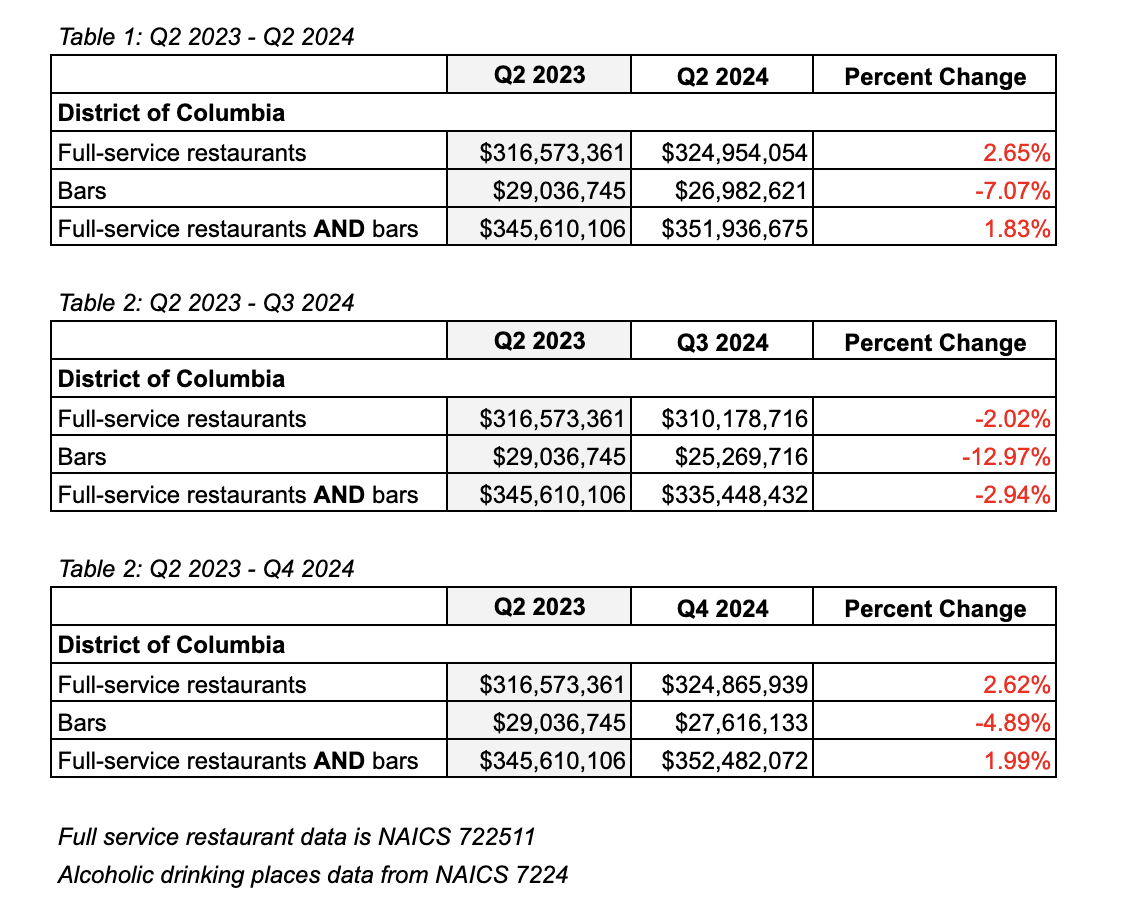
\includegraphics[width=0.75\linewidth,height=0.75\textheight]{./Images/QrtlyEarnings_Table} \end{center}

\emph{Data Source: Quarterly Census of Employment and Wages; \n Chart
Source: Author, formatted in Google Sheets.}

For full-service restaurants, total quarterly earnings increased between
Q2 2023 and Q2 2024, dipped in Q3 2024, but then rose again in Q4 2024.
Over the course of a year and a half, total quarterly earnings rose by
\$8.2 million.

Interestingly, total quarterly earnings at bars dipped \$1.4 million
over the same period. The sector as a whole shows an increase from Q2
2023 -- Q4 2024, but the diverging trend for bars in comparison to
full-service restaurants could indicate an area for further analysis.

Charts aside, we should note that there's varying testimony from DC
service workers on this issue.\footnote{Amanda Michelle Gomez, ``One
  Year In, Here's How Initiative 82 Is Affecting D.C. Restaurant
  Workers'', \emph{DCist},
  \url{https://dcist.com/story/23/12/12/initiative-82-one-year-later-dc-restaurant-worker-wages-service-charges/}}
EPI has compiled clips from a DC Council hearing where service workers
attested to economic struggles in recent months, implying that I82 may
be to blame.\footnote{Employment Policies Institute, \emph{Supercut: DC
  Council Hearing on Initiative 82 Consequences},
  \url{https://www.youtube.com/watch?v=xtxE5X1Uj7E}} However, One Fair
Wage has collected testimony with the exact opposite
sentiment.\footnote{One Fair Wage, ``The Sky Is Not Falling; The Floor
  Is Rising'',
  \url{https://static1.squarespace.com/static/6374f6bf33b7675afa750d48/t/65551d0897043249c7c1293b/1700076810648/OFW_OneYearAfter_DC82+\%281\%29.pdf},
  pg 9-13} In addition, the service workers' union Unite Local 25
maintains that I82 brings benefits to workers. Representatives from both
organizations have repeatedly pushed back on the idea of repealing I82
in response to broader economic concerns, saying this would wrongly
punish workers for the state of the economy\footnote{Kenneth Quinnell
  and Sydney Roberts, ``Service \& Solidarity Spotlight: UNITE HERE
  Local 25 Fights Effort to Reverse Restaurant Worker Wage Increases'',
  \emph{ALF-CIO},
  \url{https://aflcio.org/2025/6/6/service-solidarity-spotlight-unite-here-local-25-fights-effort-reverse-restaurant-worker}}

\subsection{Impacts on Consumers}\label{impacts-on-consumers}

How much has consumer spending in DC changed in response to increased
restaurant prices?

Already, many restaurants in DC have raised prices or added ``service
charges'' to their bills to help fund the new \$10 tipped minimum wage.
The service charges are not meant to stand in for tips, and customers
are expected to tip on top of these charges -- an expectation which has
caused confusion among locals and visitors alike.\footnote{One Fair
  Wage, ``The Sky Is Not Falling; The Floor Is Rising'',
  \url{https://static1.squarespace.com/static/6374f6bf33b7675afa750d48/t/65551d0897043249c7c1293b/1700076810648/OFW_OneYearAfter_DC82+\%281\%29.pdf},
  pg 8}

It's possible this has already led to changes in spending patterns. In
addition, DC consumers are facing higher prices at the grocery store,
and many are experiencing income instability from mass layoffs of
federal workers. RAMW has cited survey data indicating that sales have
already lowered, restaurants are reporting less diners, and District
residents are put off by higher prices.\footnote{Restaurant Association
  of Metropolitan Washington,``SURVEY: MORE THAN 2 IN 5 CASUAL DINING
  RESTAURANTS LIKELY TO CLOSE THIS YEAR'',
  \url{https://wjla.com/resources/pdf/8a0c7346-9a1e-4a24-aa42-370aa1ed705d-03182025RAMWSpringMemberSurveyFindings.pdf},
  pg 2}

For further insights, I tried to look outside local survey data.
Consumer impacts are one area not covered by the Quarterly Census of
Employment Wages (QCEW), so I explored some alternative courses.

According to the Economic Research Service, DC residents spent an
average of \$3,832 on food away from home in 2024.\footnote{USDA
  Economic Research Service, \emph{State Food Expenditure Series},
  \url{https://public.tableau.com/shared/KKC2DMMXY}?:display\_count=n\&:origin=viz\_share\_link\&:embed=y}
The ERS State Food Expenditure Series tracks consumer spending on food
in the US and compares state spending patterns to national trends. As
shown in the graph below, spending on food away from home in DC has
continued to climb since the end of the pandemic, even surpassing
pre-pandemic levels.

\begin{center}\includegraphics[width=0.75\linewidth,height=0.75\textheight]{./Images/ERS_FoodExpenditure_Table} \end{center}

\emph{Data and Chart Source: USDA Economic Resource Service, Food
Expenditure Series}

However, this data source alone did not provide decisive insights, since
``food away from home'' includes limited-service restaurants, mobile
food vendors, and other food contractors -- which are not impacted by
I82 -- in addition to full-service restaurants.

One Fair Wage (OFW), a non-profit that advocates for the end of the
tipped minimum wage, has used income data to draw conclusions about DC
tipping practices. In a November 2023 report on I-82, OFW shared data
from Square showing that workers' earnings including tips have been
increasing at a faster annual rate than base pay in recent
years:\footnote{One Fair Wage, ``The Sky Is Not Falling; The Floor Is
  Rising'',
  \url{https://static1.squarespace.com/static/6374f6bf33b7675afa750d48/t/65551d0897043249c7c1293b/1700076810648/OFW_OneYearAfter_DC82+\%281\%29.pdf},
  pg 7}

\begin{center}\includegraphics[width=0.75\linewidth,height=0.75\textheight]{./Images/OneFairWage_Earnings_Table} \end{center}

\emph{Data Source: Square Payroll Index (Oct 2023); \n Chart Source: One
Fair Wage, The Sky is Not Falling; The Floor is Rising, pg 7}

As mentioned in the report, this would indicate that customer tipping
has not been affected by price pressures so far, since earnings are
growing on top of the higher base wages.

Further analysis of DC-specific data would be helpful to assess how
elastic consumer spending and tipping are over a longer period. DC
residents face economic uncertainty in 2025, and it's possible that
anecdotal evidence will continue to indicate intentions to decrease
expenditures.

\section{Conclusion}\label{conclusion}

From my brief dive into the data, we can pinpoint some trends among each
of the impacted groups:

\begin{itemize}
\tightlist
\item
  \textbf{Restaurants and bars:} The most recent data does not seem to
  show major signs of decline in the full-service restaurant industry,
  though anecdotal evidence of closures has proliferated in 2025.
\item
  \textbf{Service workers:} Employment levels for service workers dipped
  slightly between May 2023 and Sept 2024, but total earnings for
  service workers in DC increased through the end of 2024, with the
  exception of earnings for service workers in alcoholic drinking places
  and bars (NAICS code 7224).
\item
  \textbf{Consumers:} Despite confusion over service charges at
  restaurants, available data does not indicate a significant drop off
  in spending or tipping as of the end of 2024.
\end{itemize}

However, the main purpose of this analysis was to provide a quick look
at some of the conclusions being drawn and to highlight how data can be
presented differently to support different conclusions.

It's likely too early to make conclusive statements about impacts from
I82 overall. There are a number of confounding factors, and the data
reflects a relatively short time period from which to make causal
conclusions.

One question that may come up in future analyses is the extent to which
industry change is an expected side effect of the policy. In some cases,
restaurant closures, re-openings, and employment fluctuations might be a
necessary reality as the industry adjusts to new models, prices, and
practices that allow it to pay employees a livable wage.

At the same time, it's important to continue looking at anecdotal
evidence in the context of historical, regional, and national economic
trends to determine the real scale of impacts. With such a short time
frame since implementation, and the widely acknowledged need for
industry adaptation, it would feel unfortunate for the DC Council to
decide prematurely that a healthy local economy and a minimum wage for
service workers are mutually exclusive realities.

\end{document}
